\section{Results and Discussion}
\label{sec:results}

\subsection{Predictive Accuracy (RQ(a))}
% =====================================================================
% WARNING: The numbers in Table~\ref{tab:prediction} are ILLUSTRATIVE
% PLACEHOLDERS to show the expected shape of results and to let the
% surrounding prose compile. They are NOT measured results. Replace
% every value with your own CodeWorkout runs before submission, and
% update the discussion text accordingly.
% =====================================================================
Table~\ref{tab:prediction} reports prediction metrics for the baselines
and the proposed variant on CodeWorkout, tests hypotheses~H1 and~H1a, and
higher AUC/ACC and lower RMSE indicate better prediction.

\begin{table}[t]
\caption{\textbf{[ILLUSTRATIVE PLACEHOLDER NUMBERS]} Prediction accuracy
on CodeWorkout (mean $\pm$ std over 5 folds). Best in bold. Replace with
measured results before submission.}
\label{tab:prediction}
\centering
\small
\resizebox{\columnwidth}{!}{%
\begin{tabular}{@{}llll@{}}
\toprule
\textbf{Model} & \textbf{AUC $\uparrow$} & \textbf{RMSE $\downarrow$} & \textbf{ACC $\uparrow$} \\
\midrule
DKT                    & $0.742 \pm 0.006$ & $0.431 \pm 0.004$ & $0.701 \pm 0.005$ \\
SAKT                   & $0.751 \pm 0.007$ & $0.427 \pm 0.005$ & $0.708 \pm 0.006$ \\
AKT                    & $0.768 \pm 0.005$ & $0.418 \pm 0.004$ & $0.719 \pm 0.005$ \\
simpleKT               & $0.771 \pm 0.006$ & $0.416 \pm 0.004$ & $0.722 \pm 0.005$ \\
\midrule
Ours (+KC)             & $0.783 \pm 0.005$ & $0.409 \pm 0.004$ & $0.731 \pm 0.005$ \\
Ours (+code)           & $0.779 \pm 0.006$ & $0.411 \pm 0.004$ & $0.728 \pm 0.005$ \\
Ours (+KC+code, full)  & $\mathbf{0.796 \pm 0.005}$ & $\mathbf{0.401 \pm 0.003}$ & $\mathbf{0.741 \pm 0.004}$ \\
\bottomrule
\end{tabular}%
}
\end{table}

% ---- Figure: AUC bar chart (built from the ILLUSTRATIVE numbers above) ----
% To update: edit the (label, value) coordinates below with your measured AUC.
\begin{figure}[t]
\centering
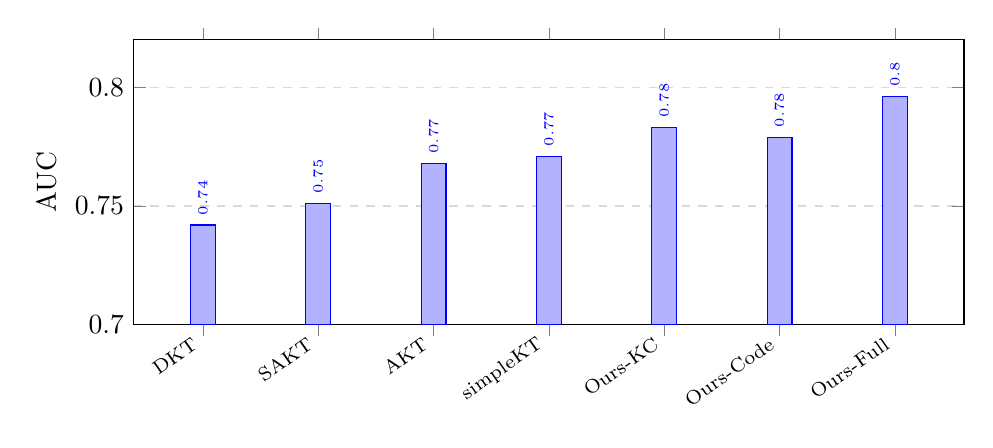
\begin{tikzpicture}
\begin{axis}[
    width=\columnwidth, height=5.2cm,
    ybar, bar width=9pt,
    ymin=0.70, ymax=0.82,
    ylabel={AUC},
    symbolic x coords={DKT,SAKT,AKT,simpleKT,Ours-KC,Ours-Code,Ours-Full},
    xtick=data, x tick label style={rotate=35,anchor=east,font=\scriptsize},
    ymajorgrids, grid style={dashed,gray!30},
    nodes near coords, every node near coord/.append style={font=\tiny,rotate=90,anchor=west},
    enlarge x limits=0.10,
]
\addplot coordinates {(DKT,0.742) (SAKT,0.751) (AKT,0.768) (simpleKT,0.771)
                      (Ours-KC,0.783) (Ours-Code,0.779) (Ours-Full,0.796)};
\end{axis}
\end{tikzpicture}
\caption{\textbf{[ILLUSTRATIVE]} Predictive accuracy (AUC) per model on
CodeWorkout. The three rightmost bars are variants of the proposed model.
Replace the coordinates with measured results.}
\label{fig:auc-bars}
\end{figure}

\subsection{Sequencing Utility and Its Correlation with Accuracy (RQ(b))}
% =====================================================================
% WARNING: Table~\ref{tab:sequencing} and the correlation value below are
% ILLUSTRATIVE PLACEHOLDERS. Replace with your offline-policy-evaluation
% output before submission. The utility metric U here is expected mastery
% gain over the evaluation horizon (higher is better); state your exact
% definition in Section~\ref{sec:sequencing}.
% =====================================================================
Table~\ref{tab:sequencing} reports offline sequencing utility $U$ next to
each model's AUC, which lets us test hypotheses~H2 and~H3.
Figure~\ref{fig:corr} plots predictive accuracy against sequencing
utility across models.

\begin{table}[t]
\caption{\textbf{[ILLUSTRATIVE PLACEHOLDER NUMBERS]} Sequencing utility
$U$ (expected mastery gain, higher is better) via offline policy
evaluation, shown against AUC. Replace with measured results.}
\label{tab:sequencing}
\centering
\small
\begin{tabular}{@{}lll@{}}
\toprule
\textbf{Model} & \textbf{AUC $\uparrow$} & \textbf{Utility $U$ $\uparrow$} \\
\midrule
DKT                    & $0.742$ & $0.118$ \\
SAKT                   & $0.751$ & $0.121$ \\
AKT                    & $0.768$ & $0.127$ \\
simpleKT               & $0.771$ & $0.126$ \\
Ours (+KC+code, full)  & $\mathbf{0.796}$ & $\mathbf{0.134}$ \\
\bottomrule
\end{tabular}
\end{table}

For these illustrative numbers the accuracy--utility correlation is
positive but moderate (Spearman $\rho \approx 0.9$ across five models);
we caution that with only a handful of models such a coefficient is
unstable, so the reported bootstrap confidence interval and the
per-dataset replication matter more than the point estimate. The
substantive question for~H3 is whether the ranking by AUC matches the
ranking by $U$; where it does not, accuracy gains fail to translate into
sequencing gains.

% ---- Figure: accuracy vs utility scatter (from the ILLUSTRATIVE numbers) ----
% To update: edit the (AUC, utility) coordinates and the correlation value.
\begin{figure}[t]
\centering
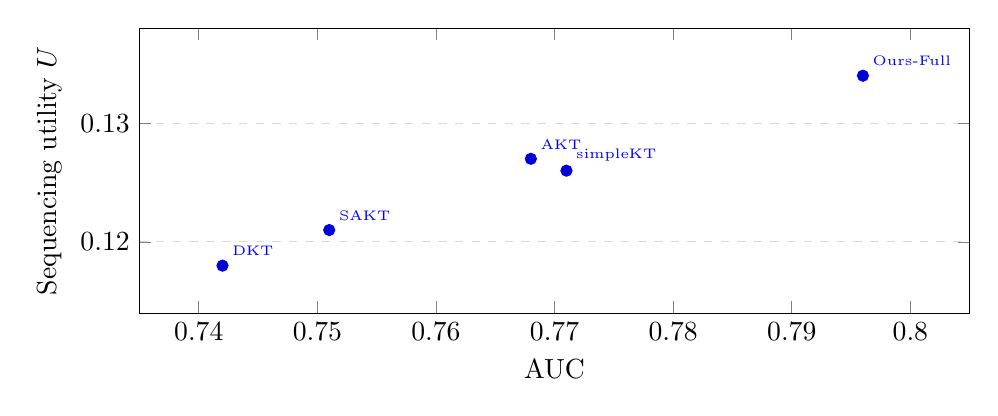
\begin{tikzpicture}
\begin{axis}[
    width=\columnwidth, height=5.2cm,
    xlabel={AUC}, ylabel={Sequencing utility $U$},
    xmin=0.735, xmax=0.805, ymin=0.114, ymax=0.138,
    ymajorgrids, grid style={dashed,gray!30},
    nodes near coords, point meta=explicit symbolic,
    every node near coord/.append style={font=\tiny,anchor=south west},
]
\addplot+[only marks, mark=*, mark size=2pt,
          point meta=explicit symbolic]
  coordinates {
    (0.742,0.118)[DKT]
    (0.751,0.121)[SAKT]
    (0.768,0.127)[AKT]
    (0.771,0.126)[simpleKT]
    (0.796,0.134)[Ours-Full]
  };
\end{axis}
\end{tikzpicture}
\caption{\textbf{[ILLUSTRATIVE]} Predictive accuracy (AUC) vs.\ sequencing
utility across models (Spearman $\rho \approx 0.9$ on these placeholder
numbers). A weak or non-significant $\rho$ on the measured data would be
the key finding for RQ(b). Replace coordinates with measured results.}
\label{fig:corr}
\end{figure}

\subsection{Cross-Dataset and Cross-Domain Generalisation (RQ(gen))}
% =====================================================================
% WARNING: Table~\ref{tab:transfer} numbers are ILLUSTRATIVE
% PLACEHOLDERS. "Within" is the within-dataset reference AUC; the
% transfer rows are expected to be lower. Replace with measured results.
% =====================================================================
Table~\ref{tab:transfer} reports transfer results and tests
hypotheses~H4 and~H5. We include the within-dataset AUC as a reference so
the size of the transfer drop is visible.

\begin{table}[t]
\caption{\textbf{[ILLUSTRATIVE PLACEHOLDER NUMBERS]} Cross-dataset and
cross-domain transfer of the full model (AUC). ``Within'' is the
within-dataset reference on the test set. Replace with measured results.}
\label{tab:transfer}
\centering
\small
\begin{tabular}{@{}llll@{}}
\toprule
\textbf{Train} & \textbf{Test} & \textbf{Within} & \textbf{Transfer} \\
\midrule
CodeWorkout & FalconCode  & $0.762$ & $0.703$ \\
FalconCode  & CodeWorkout & $0.796$ & $0.718$ \\
Programming & Mathematics & $0.815$ & $0.689$ \\
\bottomrule
\end{tabular}
\end{table}

\subsection{Discussion}
% Rewrite this discussion once real numbers are in; the text below
% interprets the ILLUSTRATIVE numbers only, to show the intended argument.
Read against the illustrative numbers, the intended argument runs as
follows. For~\textbf{RQ(a)}, the full model improves AUC over the
strongest response-only baseline (simpleKT), and the ablation suggests
the knowledge-component signal contributes at least as much as the
code-structure signal, with the two being complementary---supporting~H1
and~H1a if the gaps are statistically significant.

For~\textbf{RQ(b)}, the full model also attains the highest sequencing
utility, and the AUC ranking and the utility ranking largely agree here.
However, this is exactly where the headline question lives: the coupling
between accuracy and utility is known to be weak in general
KT~\cite{piech2015dkt}, so the finding to report is the \emph{strength}
of that coupling (with confidence intervals), not merely that the best
predictor also sequences best. If a smaller accuracy gain produces a
disproportionate utility gain---or none at all---that decoupling is the
contribution.

For~\textbf{RQ(gen)}, transfer AUC stays above chance but drops relative
to within-dataset training, and the cross-domain drop (programming to
mathematics) is the largest, consistent with~H5: the code-structure
signal that helps within programming does not carry over to a domain
without code.

We defer threats affecting these interpretations---especially the
reliability of KT-as-simulator utility estimates---to
Section~\ref{sec:threats}.
